\chapter{Lattice Concepts and Organization}
\label{c:lat.concepts}

This chapter presents the basic concepts, such as \vn{element},
\vn{branch}, and \vn{lattice}, that \bmad uses to describe such things
as LINACs, storage rings, X-ray beam lines, etc.  In fact, \bmad is
capable of simulating a whole machine complex of interconnected parts.
This includes simulating transfer lines connected to storage rings or 
simulating interconnected colliding beam storage rings.

Chapter~\sref{c:lat.file} covers the syntax of how to construct a
lattice file for input to \bmad based programs.

%---------------------------------------------------------------------------
\section{Lattice Elements}
\label{s:element.def}

\index{element}\index{marker element}
The basic component \bmad uses to describe a machine is the
\vn{element} (also called a \vn{lattice element}).  An element can be
a physical thing like a bending magnet, a quadrupole or a Bragg
crystal, or something like a \vn{marker} element (\sref{s:mark})
that is used to mark a particular point in the machine.

\index{controller element}
Another class of element are the \vn{controller} elements
(Table~\ref{t:control.classes}) that can be used for parameter control
of other elements (\sref{c:control}).

Chapter~\sref{c:elements} lists the complete set of different element
types that \bmad knows about.

%---------------------------------------------------------------------------
\section{Lattice Branches}
\label{s:branch.def}

\index{branch}
The next level up from an \vn{element} is the \vn{branch}
(\sref{s:branching}).  A \vn{branch}, also called a \vn{lattice
branch} to distinguish it from a \vn{branch} element
(\sref{s:branch}), is just an ordered sequence of elements that a
particle will travel through. A branch can represent a LINAC, X-Ray
line, storage ring or anything else that can be represented as a
simple ordered list of elements. 

Chapter~\sref{c:sequence} shows how a \vn{branch} is defined in a
lattice file with \vn{line}, \vn{list}, and \vn{use} statements.

\index{beginning element}\index{end element}
All elements in a branch are assigned a number starting from zero. The
zeroth \vn{init_ele} (\sref{s:init.ele}) element is automatically
included in every branch and is used as a marker for the beginning of
the branch.  The zeroth element is always named \vn{BEGINNING}.
Additionally, every branch will, by default, have a final marker
element (\sref{s:mark}) named \vn{END}.

%---------------------------------------------------------------------------
\section{Lattice}
\label{s:lattice.def}

\index{lattice}
\vn{branch element} A \vn{lattice} is just an array of branches that
can be interconnected together to describe an entire machine complex.
The array of \vn{branches} in a \vn{lattice} is numbered starting from
zero.

Branches can be interconnected in one of two ways: \vn{branch} and
\vn{photon_branch} elements (\sref{s:branch}) may be used to simulate
forking beam lines (\sref{s:branching}) such as what occurs when there
is a dump line connection or an X-ray beam line which is connected to
a wiggler or undulator. Additionally, \vn{multipass} lines
(\sref{s:multipass}) can be used to simulate branches that share
common elements such as the interaction region in colliding beam
machines.

%---------------------------------------------------------------------------
\section{Lord and Slave Elements}
\label{s:lattice}

\begin{figure}[tb]
 \begin{center}
 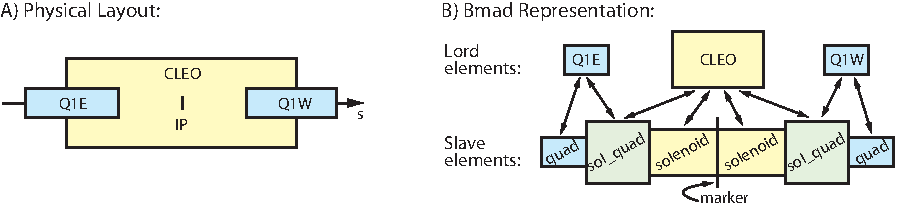
\includegraphics[width=6.0in]{superimpose-ip.pdf}
 \caption[Superposition example.]
 {
Superposition Example. A) Interaction region layout
with quadrupoles overlapping a solenoid. B) The Bmad lattice
representation has a list of split elements to track through and the
undivided ``lord'' elements. Pointers (double headed arrows), keep
track of the correspondence between the lords and their slaves.
 }
 \label{f:super.ip}
 \end{center}
 \end{figure}

%---------------------------------------------------------------------------

A real machine is more than a collection of independent lattice
elements. For example, the field strength in a string of elements may
be tied together via a common power supply, or the fields of different
elements may overlap.

\bmad tries to capture these interdependencies using what are referred
to as \vn{lord} and \vn{slave} elements. The \vn{lord} elements may be
divided into two classes. In one class are the \vn{controller}
elements.  These are \vn{overlay} (\sref{s:overlay}), \vn{group}
(\sref{s:group}), and \vn{girder} (\sref{s:girder}) elements that
control the attributes of other elements which are their slaves.

The other class of \vn{lord} elements embody the separation of the
physical element from the track that a particle takes when it passes
through the element. An example will make this clear.
\vn{Superposition} (\sref{s:super}) is the ability to overlap lattice
elements spatially. \fig{f:super.ip} shows an example which is a
greatly simplified version of the IR region of Cornell's CESR storage
ring when CESR was an e+/e-- collider. As shown in \fig{f:super.ip}A,
two quadrupoles named \vn{q1w} and \vn{q1e} are partially inside and
partially outside the interaction region solenoid named \vn{cleo}. In
the lattice file, the IR region layout is defined to be
 {\small
\begin{example}
  cesr: line = (... q1e, dft1, ip, dft1, q1w ...)
  cleo: solenoid, l = 3.51, superimpose, ref = ip
\end{example}
 }
The line named \vn{cesr} ignores the solenoid and just contains the
interaction point marker element named \vn{ip} which is surrounded by
two drifts named \vn{dft1} which are, in turn, surrounded by the
\vn{q1w} and \vn{q1e} quadrupoles. The solenoid is added to the layout
on the second line by using superposition. The ``ref = ip'' indicates
that the solenoid is placed relative to \vn{ip}. The default, which is
used here, is to place the center of the superimposed \vn{cleo}
element at the center of the \vn{ip} reference element.  The
representation of the lattice in \bmad will contain two branch
\vn{sections} (``sections'' is explained more fully later): One
section, called the \vn{tracking section}, contains the elements that
are needed for tracking particles. In the current example, as shown in
\fig{f:super.ip}B, the first IR element in the tracking section is a
quadrupole that represents the part of \vn{q1e} outside of the
solenoid. The next element is a combination solenoid/quadrupole,
called a \vn{sol_quad}, that represents the part of \vn{q1e} inside
\vn{cleo}, etc.  The other branch section that Bmad creates is called
the \vn{lord section} This section contain the undivided ``physical''
\vn{super_lord} elements (\sref{s:super}) which, in this case are
\vn{q1e}, \vn{q1w}, and \vn{cleo}. Pointers are created between the
lords and their \vn{super_slave} elements in the tracking section so
that changes in parameters of the lord elements can be transferred to
their corresponding slaves.

\vn{super_lord}s are used when there are overlapping fields between
elements, the other case where there is a separation between the
physical element and the particle track comes when a particle passes
through the same physical element multiple times such as in an Energy
Recovery Linac or where different beams pass through the same element
such as in an interaction region. In this case, \vn{multipass_lords}
representing the physical element and \vn{multipass_slaves}
representing the track can be constructed (\sref{s:multipass}).
Superposition and multipass can be combined in situations where there
are overlapping fields in elements where the particle passes through

For historical reasons, each \vn{branch} in a lattice has a
\vn{tracking section} and a \vn{lord section} and the \vn{tracking
section} is always the first (lower) part of the element array and the
\vn{lord section} inhabits the second (upper) part of the array.  All
the \vn{lord} elements are put in the \vn{lord section} of branch 0
and all the other \vn{lord sections} of all the other branches are
empty.

As a side note, Etienne Forest's PTC code (\sref{s:ptc}) uses separate
structures to separate the physical element, which PTC calls an
\vn{element} from the particle track which PTC call a \vn{fibre}.
[Actually, PTC has two structures for the physical element,
\vn{element} and \vn{elementp}. The latter being the ``polymorph''
version.] This \vn{element} and \vn{fibre} combination corresponds to
\bmad \vn{multipass_lord} and \vn{multipass_slave} elements. PTC does
not handle overlapping fields.

